% Intended LaTeX compiler: pdflatex
\documentclass[10pt,a4paper,UTF8]{article}
\usepackage{zclorg}
\usepackage{tikztheorem}
\author{zcl.space}
\date{}
\title{指数分布}
\hypersetup{
 pdfauthor={zcl.space},
 pdftitle={指数分布},
 pdfkeywords={probability},
 pdfsubject={},
 pdfcreator={Emacs 25.0.50.1 (Org mode 9.0.6)},
 pdflang={English}}
\begin{document}

\maketitle
\tableofcontents
\titlepic{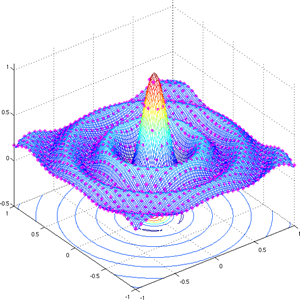
\includegraphics[scale=0.25]{../../img/sinc.PNG}}


\section{定义}
\label{sec:org894b3c5}


如果一个连续性随机变量的密度函数如下:\(\forall \lambda > 0\),有:
\begin{equation}
\label{eq:1}
f(x) =
\begin{cases}
\lambda e^{-\lambda x} & x \geq 0 \\
0 & x < 0
\end{cases}
\end{equation}
则称该随机变量是参数为\(\lambda\)的指数分布。指数随机变量的分布函数\(F(a)\)如下:
\begin{equation}
\label{eq:2}
F(a) = P\{x \leq a\} = \int_{0}^{a}\lambda e^{-\lambda x}dx = 1 - e^{-\lambda a}, a\geq 0
\end{equation}
\section{期望和方差}
\label{sec:orgadd6b35}


令\(X\)是一参数为\(\lambda\)的指数随机变量,则\(\mathbb{E}[X]\)和\(\mathrm{Var}[X]\)的计算如下:
\begin{equation}
\label{eq:3}
\mathbb{E}[X^{n}] = \int_{0}^{\infty}x^{n}\lambda e^{-\lambda x}dx
\end{equation}

利用分部积分我们可以得到:
\begin{equation}
\label{eq:4}
\mathbb{E}[X^{n}] = \frac{n}{\lambda}\mathbb{E}[X^{n-1}]
\end{equation}
令\(n=1\)则有:
\begin{equation}
\label{eq:5}
\mathbb{E}[X] = \frac{1}{\lambda}
\end{equation}
令\(n=2\)则有:
\begin{equation}
\label{eq:6}
\mathbb{E}[X^{2}] = \frac{2}{\lambda^{2}}
\end{equation}
因此:\(\mathrm{Var}[X] = \frac{1}{\lambda^{2}}\)
即指数分布的期望恰好等于参数\(\lambda\)的倒数,而方差等于期望的平方。

在实际生活中,指数分布通常用来描述某个时间发生的等待时间的分布,例如地震发生的时间间隔;一场战争发生的时间间隔;从现在开始到你接到下一个误拨的电话的时间间隔。
\section{永远年轻的分布}
\label{sec:orge83d5dd}


我们称一个非负随机变量\(X\)是无记忆的,如果:
\begin{equation}
\label{eq:7}
P\{ X > s + t | X > t\} = P\{ X > s \}
\end{equation}
设\(X\)是某个设备的寿命,上式说明在已知该设备已经使用\(t\)小时的条件下寿命至少为\(s+t\)的概率与开始时寿命至少为\(s\)小时的概率是一样的。换句话说,如果该设备在使用\(t\)小时后还能使用,那么剩余的寿命同一开始时的寿命的分布是一样的。就好像该设备对已经使用了\(t\)小时是无记忆似的。

式 (\ref{eq:7})等效于:
\begin{equation}
\label{eq:8}
\frac{P\{X > s+t, X > t\}}{P\{X > t\}} = P\{ X > s \}
\end{equation}
可以验证指数分布就是这样的无记忆分布。指数分布也叫作永远年轻的分布。
\end{document}
